\documentclass [a4paper, 12pt] {article}
\usepackage{tikz}
\usepackage{xcolor}
\usepackage[margin = 2cm]{geometry}
\definecolor{customcolor1}{HTML}{abe0f9}
\definecolor{customcolor2}{HTML}{fee4b3}

\title{Data Structure}
\author{Pranto}
\date{\today}

\begin{document}
\maketitle
\section{Graph 4}
Lets make the Graph of ED task 4.
\begin{center}
    \vspace{10pt}
% 1st
\begin{minipage}[t]{.45555\linewidth}
    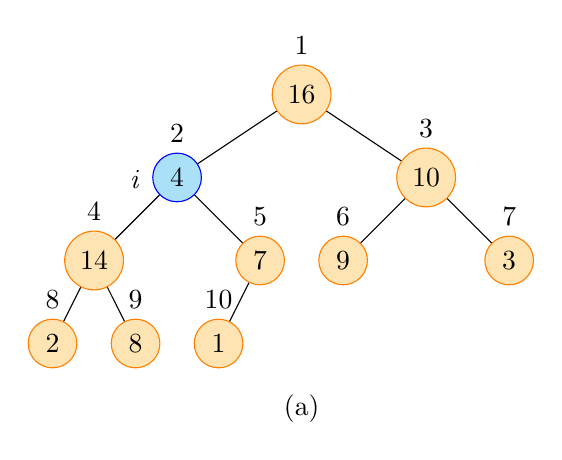
\begin{tikzpicture}[scale = 1.5]
        % Nodes
        \node [draw = orange, fill = customcolor2, circle] (a) at (0pt, 0pt) {16};
        \node [draw = blue, fill = customcolor1, circle] (b) at (-30pt, -20pt) {4};
        \node [draw = orange, fill = customcolor2, circle] (c) at (30pt, -20pt) {10};
        \node [draw = orange, fill = customcolor2, circle] (d) at (-50pt, -40pt) {14};
        \node [draw = orange, fill = customcolor2, circle] (e) at (-10pt, -40pt) {7};
        \node [draw = orange, fill = customcolor2, circle] (f) at (10pt, -40pt) {9};
        \node [draw = orange, fill = customcolor2, circle] (g) at (50pt, -40pt) {3};
        \node [draw = orange, fill = customcolor2, circle] (h) at (-60pt, -60pt) {2};
        \node [draw = orange, fill = customcolor2, circle] (i) at (-40pt, -60pt) {8};
        \node [draw = orange, fill = customcolor2, circle] (j) at (-20pt, -60pt) {1};

        % Levels
        \node [above] at (a.north) {1};
        \node [above] at (b.north) {2};
        \node [above] at (-40pt,-25pt) {\textit{i}};
        \node [above] at (c.north) {3};
        \node [above] at (d.north) {4};
        \node [above] at (e.north) {5};
        \node [above] at (f.north) {6};
        \node [above] at (g.north) {7};
        \node [above] at (h.north) {8};
        \node [above] at (i.north) {9};
        \node [above] at (j.north) {10};

        % Lines
        \draw (a) -- (b) -- (d) -- (h);
        \draw (a) -- (c) -- (g);
        \draw (b) -- (e) -- (j);
        \draw (c) -- (f);
        \draw (d) -- (i);

        % Name Level
        \node [below] at (0pt, -70pt) {(a)};

    \end{tikzpicture}
\end{minipage}
% 2nd
\begin{minipage}[t]{.45555\linewidth}
    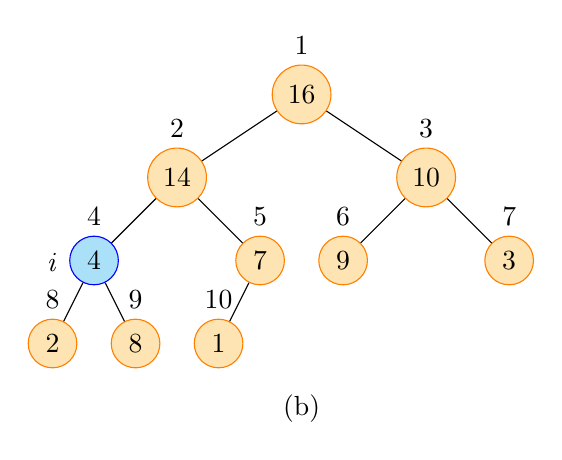
\begin{tikzpicture}[scale = 1.5]
        % Nodes
        \node [draw = orange, fill = customcolor2, circle] (a) at (0pt, 0pt) {16};
        \node [draw = orange, fill = customcolor2, circle] (b) at (-30pt, -20pt) {14};
        \node [draw = orange, fill = customcolor2, circle] (c) at (30pt, -20pt) {10};
        \node [draw = blue, fill = customcolor1, circle] (d) at (-50pt, -40pt) {4};
        \node [draw = orange, fill = customcolor2, circle] (e) at (-10pt, -40pt) {7};
        \node [draw = orange, fill = customcolor2, circle] (f) at (10pt, -40pt) {9};
        \node [draw = orange, fill = customcolor2, circle] (g) at (50pt, -40pt) {3};
        \node [draw = orange, fill = customcolor2, circle] (h) at (-60pt, -60pt) {2};
        \node [draw = orange, fill = customcolor2, circle] (i) at (-40pt, -60pt) {8};
        \node [draw = orange, fill = customcolor2, circle] (j) at (-20pt, -60pt) {1};

        % Levels
        \node [above] at (a.north) {1};
        \node [above] at (b.north) {2};
        \node [above] at (-60pt,-45pt) {\textit{i}};
        \node [above] at (c.north) {3};
        \node [above] at (d.north) {4};
        \node [above] at (e.north) {5};
        \node [above] at (f.north) {6};
        \node [above] at (g.north) {7};
        \node [above] at (h.north) {8};
        \node [above] at (i.north) {9};
        \node [above] at (j.north) {10};

        % Lines
        \draw (a) -- (b) -- (d) -- (h);
        \draw (a) -- (c) -- (g);
        \draw (b) -- (e) -- (j);
        \draw (c) -- (f);
        \draw (d) -- (i);

        % Name Level
        \node [below] at (0pt, -70pt) {(b)};

    \end{tikzpicture}
\end{minipage}
\end{center}
% 2nd
\begin{minipage}[t]{.45555\linewidth}
    \hspace{16pt}
    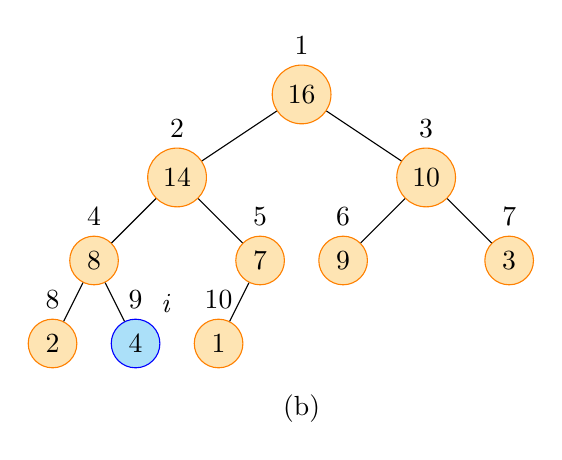
\begin{tikzpicture}[scale = 1.5]
        % Nodes
        \node [draw = orange, fill = customcolor2, circle] (a) at (0pt, 0pt) {16};
        \node [draw = orange, fill = customcolor2, circle] (b) at (-30pt, -20pt) {14};
        \node [draw = orange, fill = customcolor2, circle] (c) at (30pt, -20pt) {10};
        \node [draw = orange, fill = customcolor2, circle] (d) at (-50pt, -40pt) {8};
        \node [draw = orange, fill = customcolor2, circle] (e) at (-10pt, -40pt) {7};
        \node [draw = orange, fill = customcolor2, circle] (f) at (10pt, -40pt) {9};
        \node [draw = orange, fill = customcolor2, circle] (g) at (50pt, -40pt) {3};
        \node [draw = orange, fill = customcolor2, circle] (h) at (-60pt, -60pt) {2};
        \node [draw = blue, fill = customcolor1, circle] (i) at (-40pt, -60pt) {4};
        \node [draw = orange, fill = customcolor2, circle] (j) at (-20pt, -60pt) {1};

        % Levels
        \node [above] at (a.north) {1};
        \node [above] at (b.north) {2};
        \node [above] at (-32.5pt,-55pt) {\textit{i}};
        \node [above] at (c.north) {3};
        \node [above] at (d.north) {4};
        \node [above] at (e.north) {5};
        \node [above] at (f.north) {6};
        \node [above] at (g.north) {7};
        \node [above] at (h.north) {8};
        \node [above] at (i.north) {9};
        \node [above] at (j.north) {10};

        % Lines
        \draw (a) -- (b) -- (d) -- (h);
        \draw (a) -- (c) -- (g);
        \draw (b) -- (e) -- (j);
        \draw (c) -- (f);
        \draw (d) -- (i);

        % Name Level
        \node [below] at (0pt, -70pt) {(b)};

    \end{tikzpicture}
\end{minipage}
\end{document}